%----------------------------------------------------------------------------------------
% CHAPTER 2
%----------------------------------------------------------------------------------------
\chapter{Material and methods} % Main chapter title
\label{Chapter2}

\section{Study area}
This study was conducted within the North American Arctic tundra, specifically focusing on the Circumpolar Arctic Vegetation Map's (\cite{walker_circumpolar_2005}; \cite{walker_circumpolar_2016}) subzones C, D, and E (as depicted in Fig. \ref{fig:testsite_overview}). These subzones represent distinct bioclimatic regions across the northern Alaskan Arctic, each characterized by varying vegetation types and permafrost conditions. The vegetation across the Arctic tundra broadly comprises a mix of herbaceous plants, low shrubs, mosses, and lichens. Common plant types include dwarf shrubs, graminoids, mosses and lichens. While precise subzone-specific vegetation descriptions can vary, general trends indicate that subzone C typically features a mix of prostrate and erect dwarf shrubs alongside graminoids. Subzone D often presents as erect dwarf-shrub tundra, interspersed with sedges and mosses. In contrast, subzone E can support taller low shrubs in warmer locations, also accompanied by sedges and mosses (\cite{walker_circumpolar_2005}).

\section{Data Source}
\subsection{In-Situ data}
In-situ vegetation data for this study were acquired from the \ac{ava} (\cite{noauthor_current_nodate}). These ground-truth observations were extracted and managed using the Turboveg software (\cite{hennekens_stephan_m_turboveg_2001}). This data served to provide essential ground-based information for validation and contextualization of the hyperspectral imagery and the \ac{svh}. The plot surveys contributing to this dataset were conducted across various years, specifically 2001, 2005, 2010, 2012, 2014, and 2015. They collectively comprise 354 unique plot locations, 1261 plant species, 20 habitat types and 64 plant communities.
\subsection{Hyperspectral data}
This study utilized hyperspectral images captured by the \ac{avirisng} instrument, mounted on a Twin Otter platform (\cite{noauthor_aviris-next_nodate}). \ac{avirisng} is an advanced airborne sensor designed to provide continuous imaging spectroscopy measurements with a high signal-to-noise ratio across the solar reflected spectral range. The instrument captures spectra as images, covering a wavelength range from 380 nm to 2510 nm with 5 nm sampling intervals (\cite{miller_above_2024}). The capturing of the images was part of the \ac{nasa} \ac{above} campaign (\cite{noauthor_arctic-boreal_nodate}). For this research, the utilized images had a spectral resolution of 425 bands and a spatial resolution of 5 m. The actual images were acquired via the \ac{ornl} of the \ac{daac} (\cite{miller_above_2024}) and the flight lines were downloaded from the official \ac{jpl} data portal (https://popo.jpl.nasa.gov/).


\section{Data workflow}
Fig. \ref{fig:thesis_workflow} outlines the workflows implemented in the study. Following the initial definition of test sites, I processed the datasets with two parallel processing streams: the "Hyperspectral Data" workflow and the "Ground Data" workflow. I merged the results of both stream into one for my final analysis.
\begin{figure}[H]
    \centering
    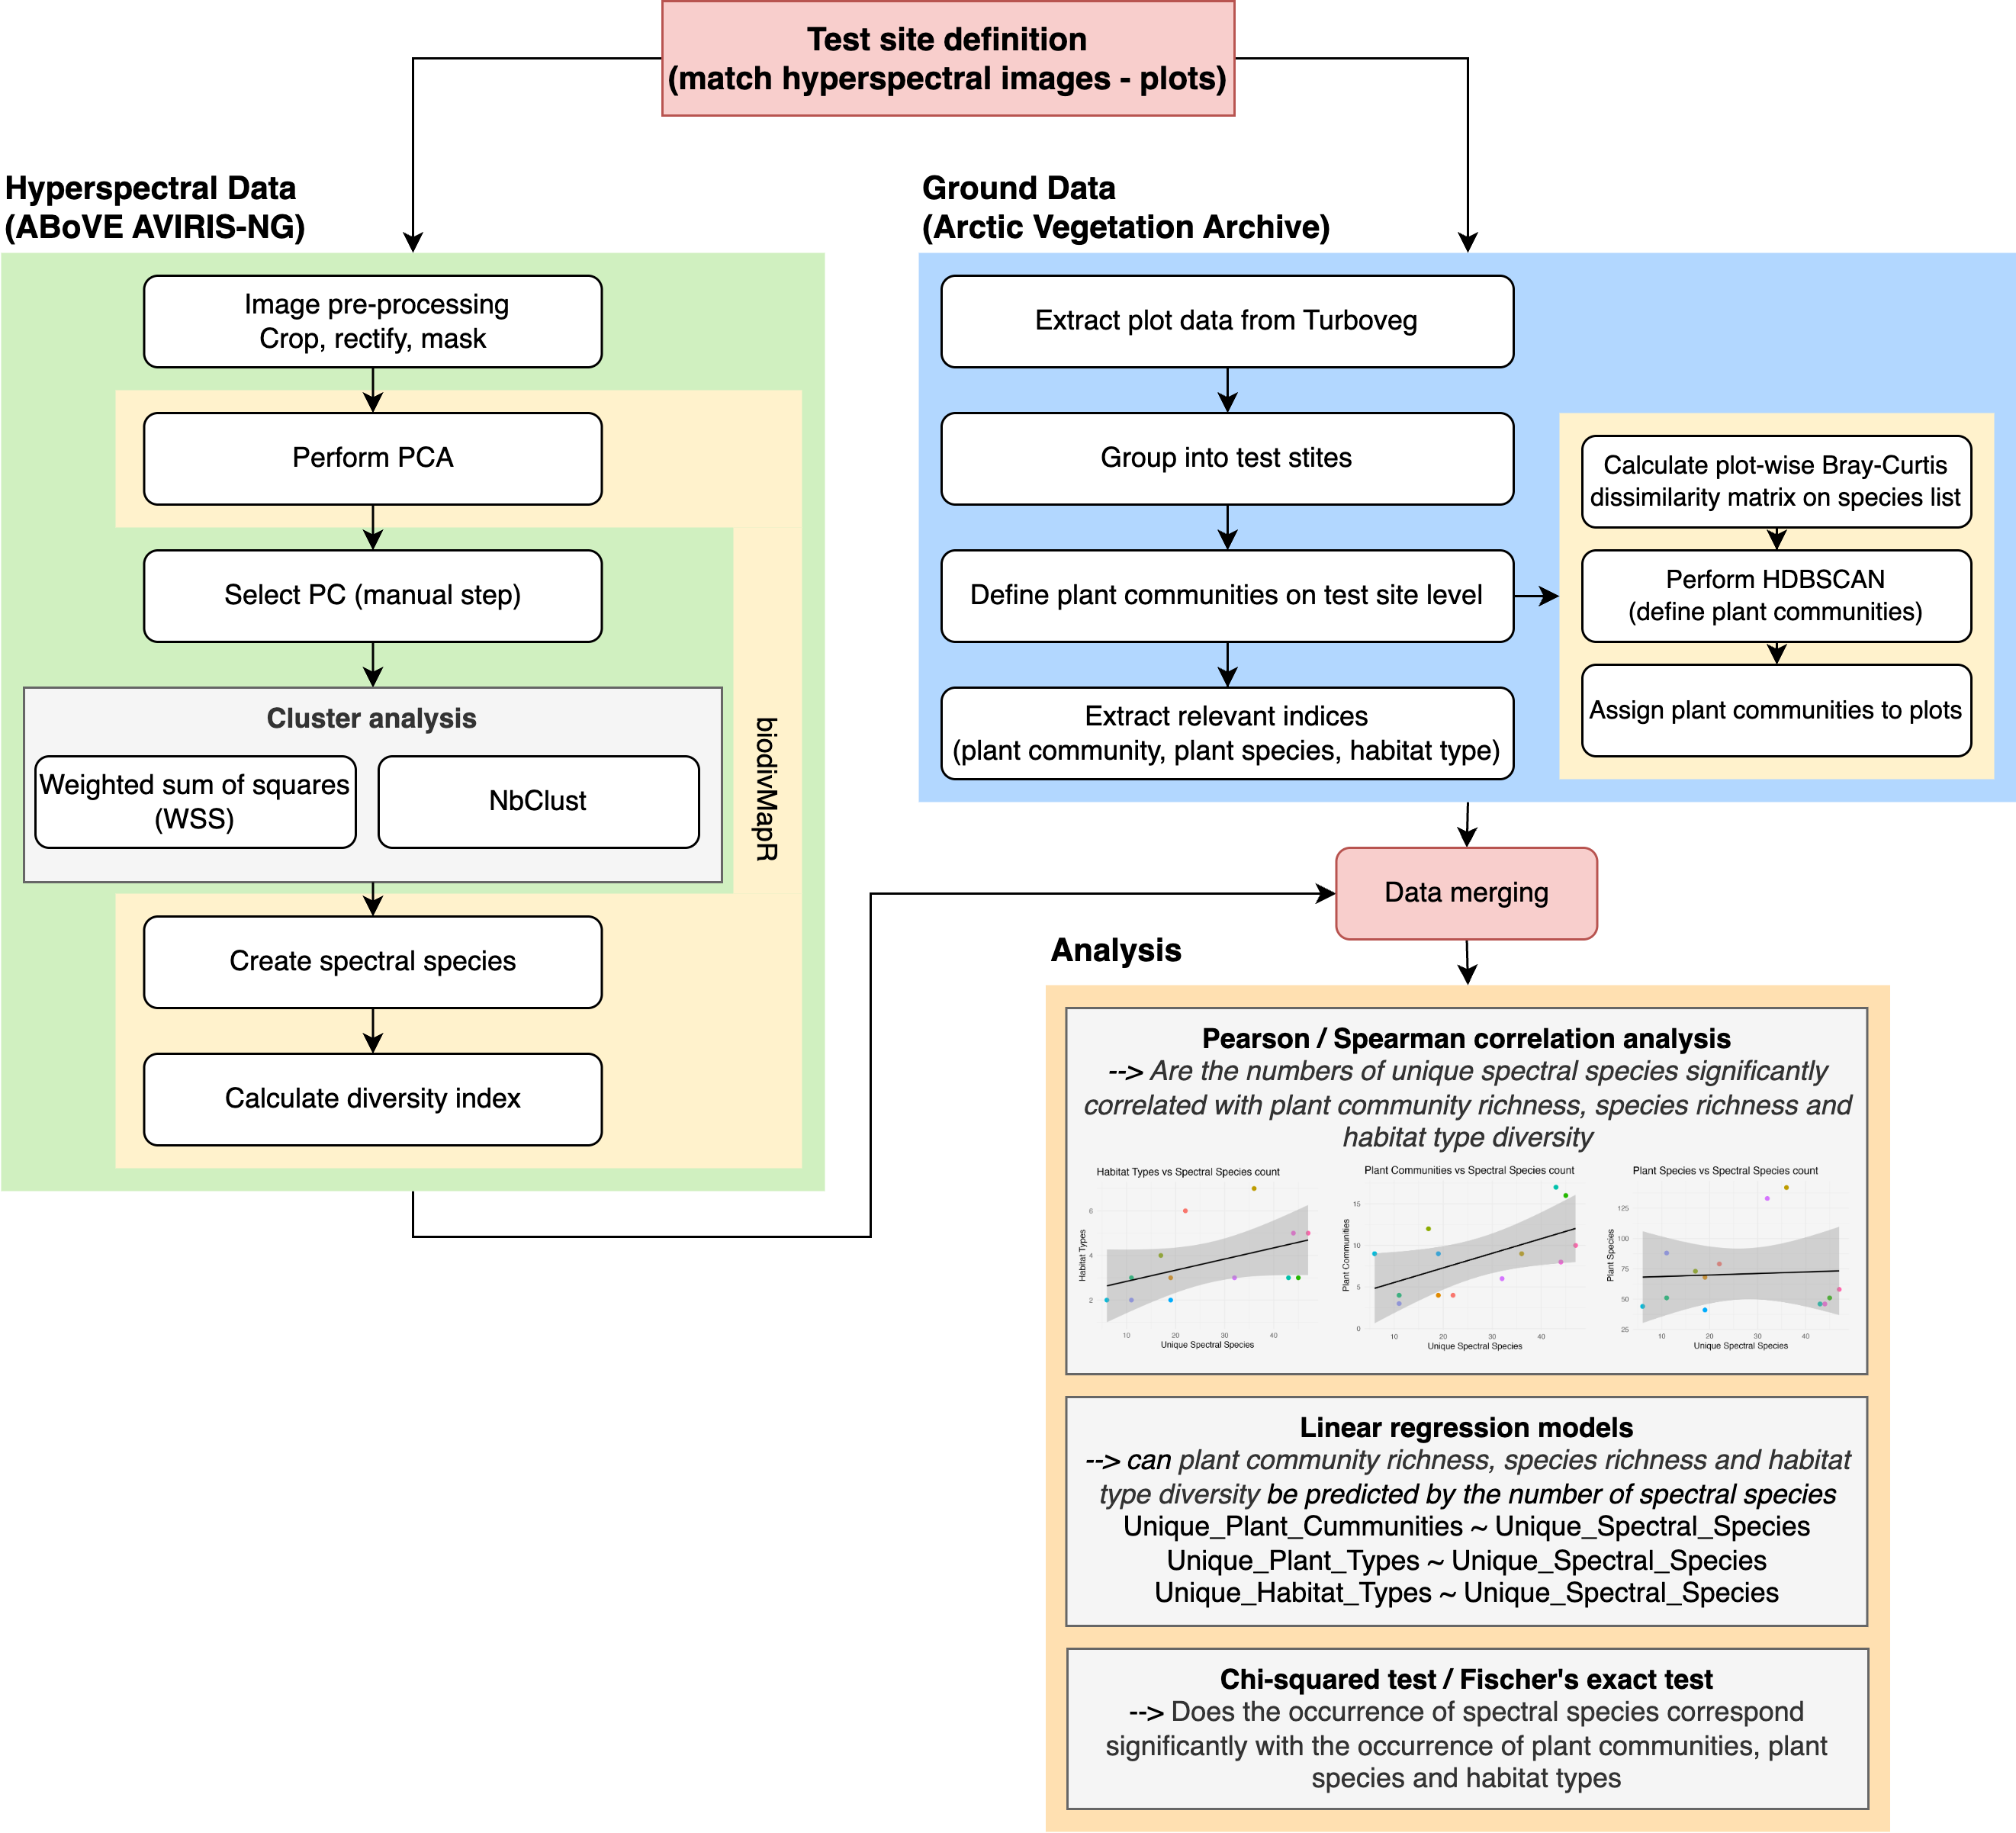
\includegraphics[width=0.9\textwidth]{Figures/WorkflowDiagram.png} % Replace with your actual image path
    \caption{Thesis workflow: This process flow diagram outlines the steps undertaken in both data streams, "Hyperspectral Data" and "Ground Data", to derive results from each. In the final stage, the outcome of the two streams are combined, allowing for statistical validation of the thesis hypothesis.}
    \label{fig:thesis_workflow}
\end{figure}

%----------------------------------------------------------------------------------------

\section{Test site definition}
To ensure the analysis included only hyperspectral imagery paired with corresponding in-situ data, I cross-referenced \ac{avirisng} flight lines with vegetation plot locations from the \ac{ava}. Further, only datasets from July and August were used, as these months presumably offer optimal vegetation coverage in the Arctic tundra. By overlaying spatial data, I identified 13 test sites, distributed across subzones C, D, and E of the northern Alaskan Arctic tundra as can be seen in Fig. \ref{fig:testsite_overview}. Additional metrics for the test sites can be seen Tab. \ref{tab:testsite_metadata}.
\begin{figure}[H]
    \centering
    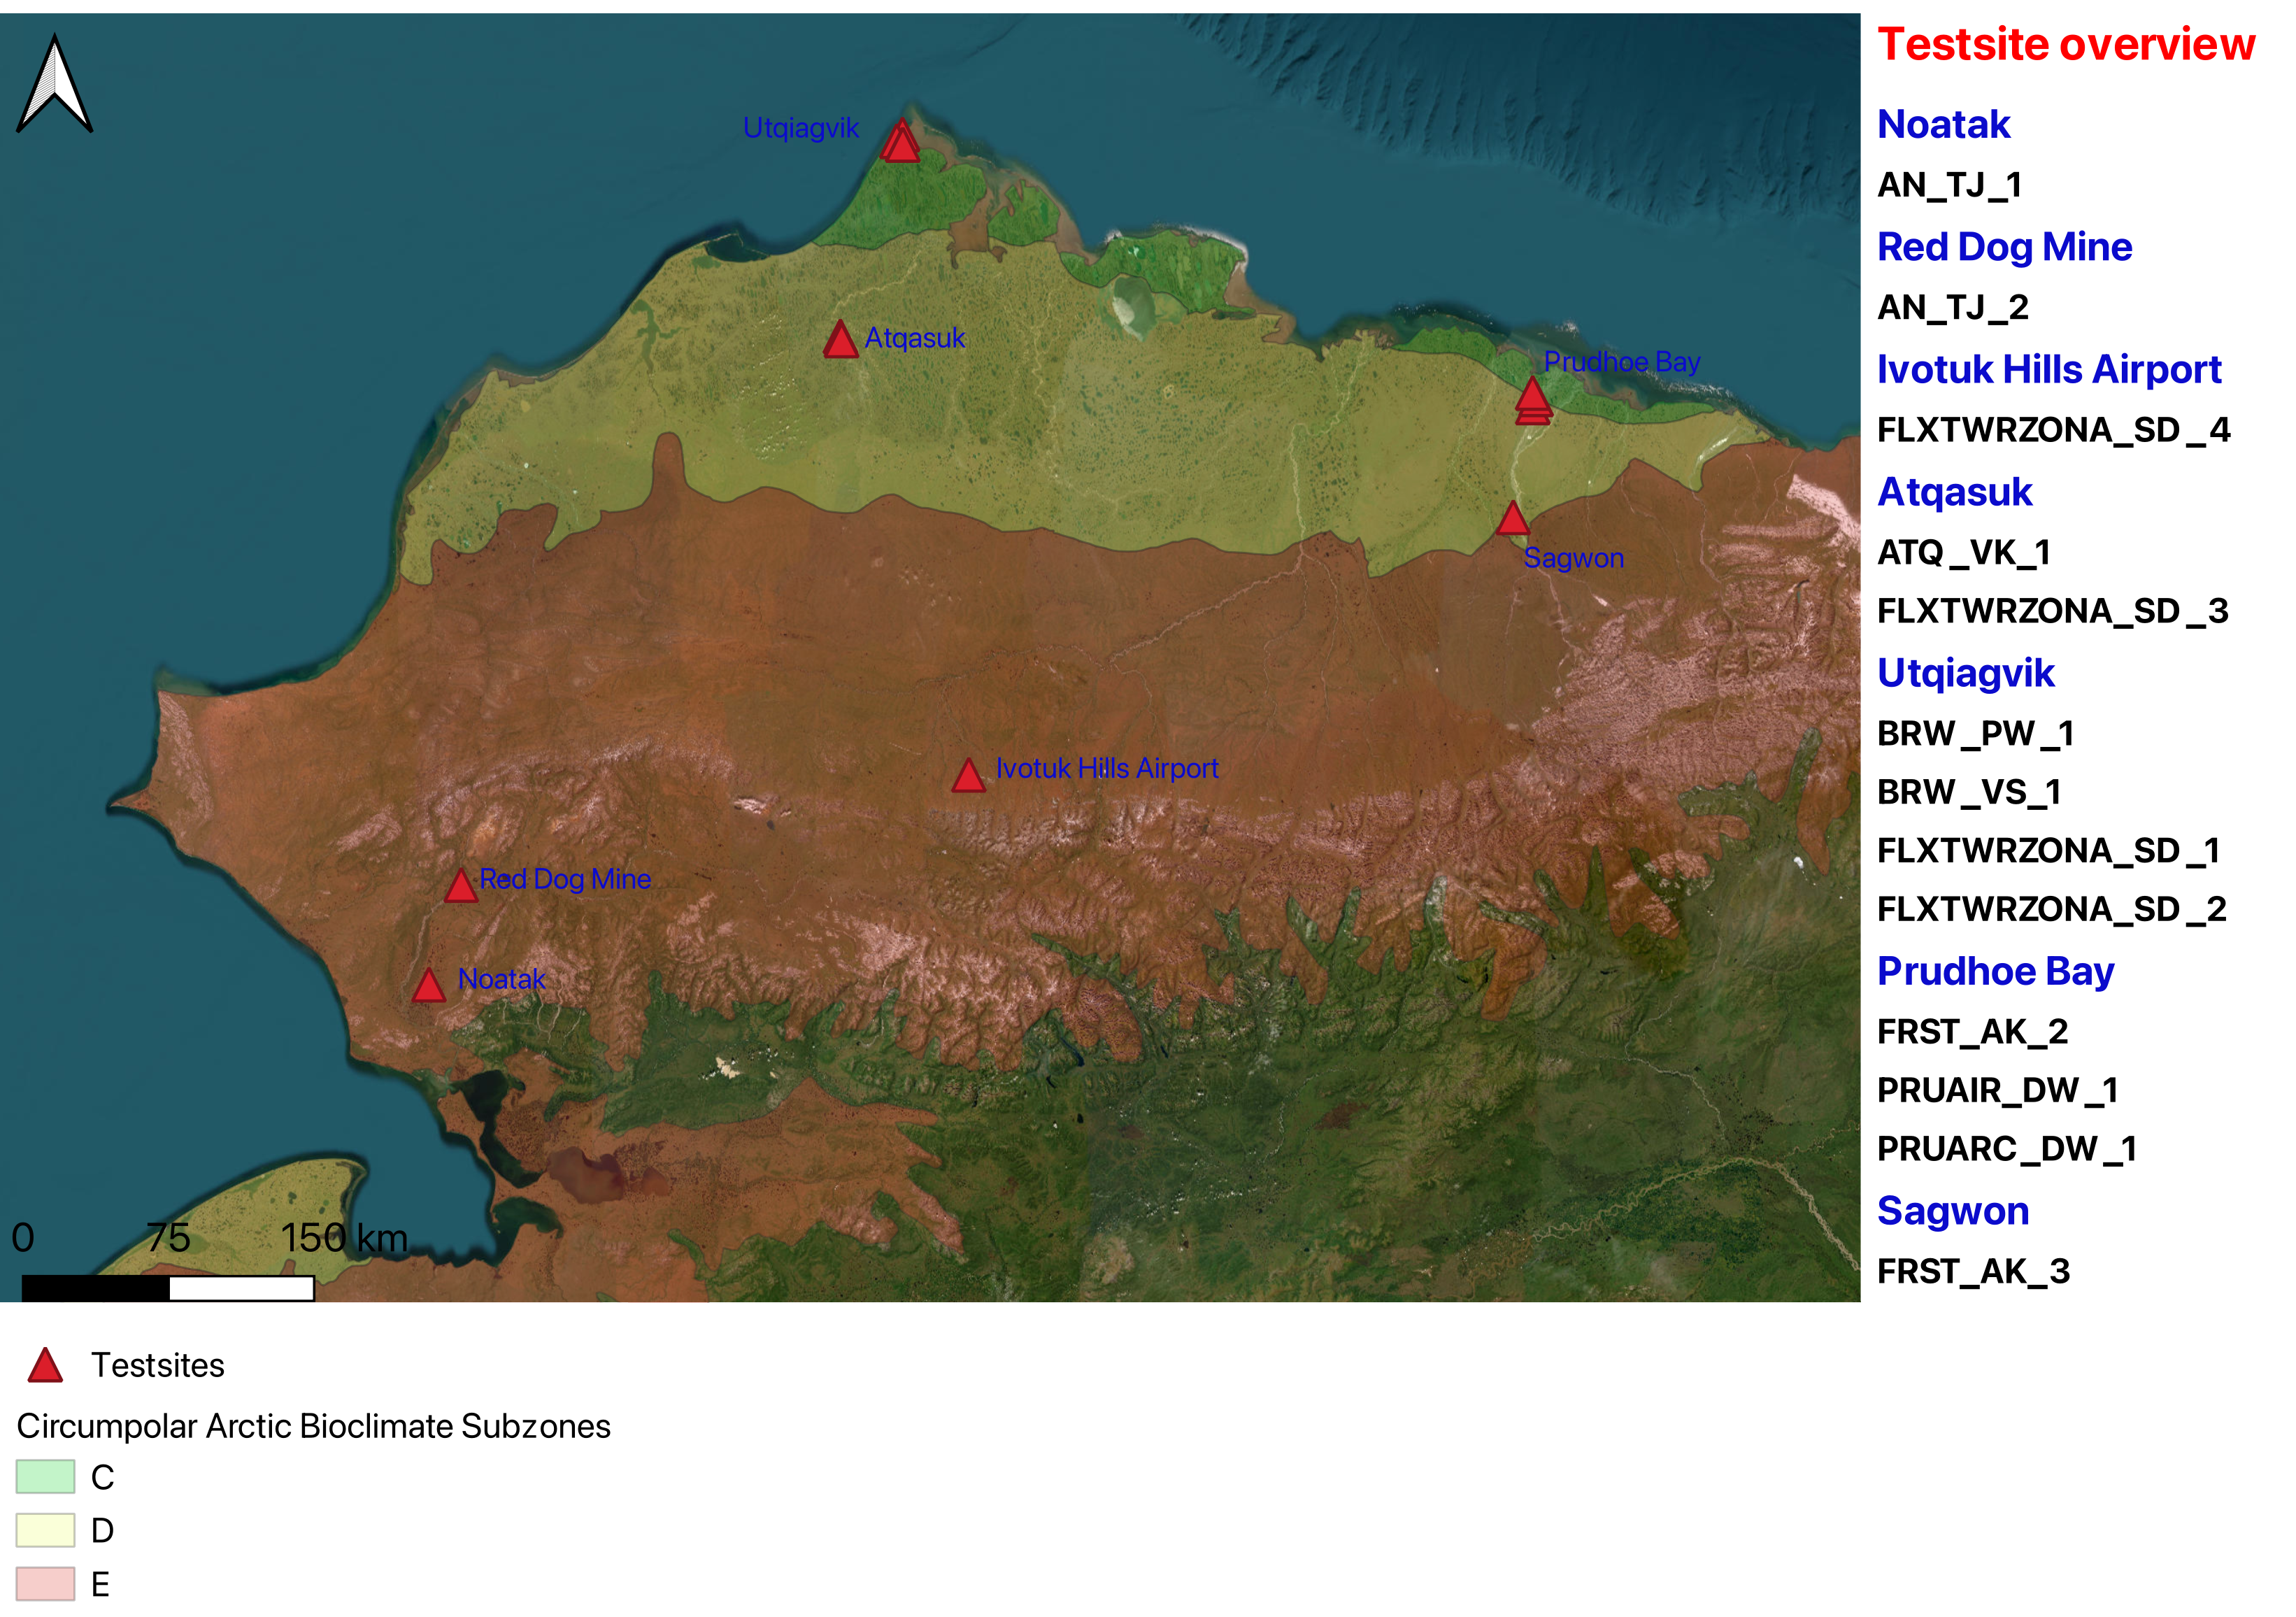
\includegraphics[width=0.9\textwidth]{Figures/TestSiteOverview.png} % Replace with your actual image path
    \caption{Map of the thirteen test sites across subzones C, D, and E of the northern Alaskan Arctic Tundra.}
    \label{fig:testsite_overview}
\end{figure}

\begin{table}[htbp]
\centering
\caption{Test sites with corresponding flight IDs, principal components retained, and site metadata. The hyperspectral images with the IDs ang20190712t231624 and ang20190712t212208 could be used for multiple test sites}
\resizebox{\textwidth}{!}{%
\begin{tabular}{lllllll}
\hline
\textbf{Test site} & \textbf{Flight ID} & \textbf{Year Flightstrip} & \textbf{Year Plots} & \textbf{Subzone} \\
\hline
AN\_TJ\_1 & \href{https://popo.jpl.nasa.gov/avng/y22/ang20220711t002111rfl.tar.gz}{ang20220711t002111}  & 2022 & 2005 & E \\
AN\_TJ\_2 & \href{https://popo.jpl.nasa.gov/avng/y22/ang20220711t003358rfl.tar.gz}{ang20220711t003358}  & 2022 & 2005 & E \\
ATQ\_VK\_1 & \href{https://popo.jpl.nasa.gov/avng/y19/ang20190712t231624rfl.tar.gz}{ang20190712t231624}  & 2019 & 2010 & D \\
BRW\_PW\_1 & \href{https://popo.jpl.nasa.gov/avng/y19/ang20190712t212208rfl.tar.gz}{ang20190712t212208}  & 2019 & 2010 & C \\
BRW\_VS\_1 & \href{https://popo.jpl.nasa.gov/avng/y19/ang20190712t212208rfl.tar.gz}{ang20190712t212208}  & 2019 & 2012 & C \\
FLXTWRZONA\_SD\_1 & \href{https://popo.jpl.nasa.gov/avng/y19/ang20190712t211646rfl.tar.gz}{ang20190712t211646}  & 2019 & 2014 & C \\
FLXTWRZONA\_SD\_2 & \href{https://popo.jpl.nasa.gov/avng/y19/ang20190712t212208rfl.tar.gz}{ang20190712t212208}  & 2019 & 2014 & C \\
FLXTWRZONA\_SD\_3 & \href{https://popo.jpl.nasa.gov/avng/y19/ang20190712t231624rfl.tar.gz}{ang20190712t231624}  & 2019 & 2014 & D \\
FLXTWRZONA\_SD\_4 & \href{https://popo.jpl.nasa.gov/avng/y19/ang20190706t210739rfl.tar.gz}{ang20190706t210739}  & 2019 & 2014 & E \\
FRST\_AK\_2 & \href{https://popo.jpl.nasa.gov/avng/y22/ang20220709t233937rfl.tar.gz}{ang20220709t233937}  & 2022 & 2001 & D \\
FRST\_AK\_3 & \href{https://popo.jpl.nasa.gov/avng/y19/ang20190713t024201rfl.tar.gz}{ang20190713t024201}  & 2019 & 2001 & D \\
PRUAIR\_DW\_1 & \href{https://popo.jpl.nasa.gov/avng/y17/ang20170709t003728rfl.tar.gz}{ang20170709t003728}  & 2017 & 2015 & C \\
PRUARC\_DW\_1 & \href{https://popo.jpl.nasa.gov/avng/y17/ang20170709t000442rfl.tar.gz}{ang20170709t000442}  & 2017 & 2014 & C \\
\hline
\end{tabular}
}
\label{tab:testsite_metadata}
\end{table}


\section{In-Situ data workflow}
Habitat type and species information were directly extracted from the Turboveg datasets, as these use standardized nomenclature. In contrast, plant community names lacked standardization and were assigned using two different classification systems: the Braun-Blanquet method and the Field Community Name method. This introduced a high degree of subjectivity from field observers. As a result, the combined dataset from all test sites contained 354 plot locations and 64 distinct plant community names. To address this inconsistency, I reclassified plant communities on the test site level using an unsupervised clustering approach. I applied \ac{hdbscan} (\cite{noauthor_how_nodate}) to the first two principal coordinates from a Bray-Curtis dissimilarity matrix based on species abundance data. Principal coordinates were extracted via \ac{pcoa} using the \fun{cmdscale} function. \ac{hdbscan} was run with a minimum points threshold of 2 to detect dense clusters while minimizing noise. Each plot was assigned a cluster ID representing a plant community, resulting in the numbers shown in Tab. \ref{tab:unique_features}, column "Unique plant communities". The result plots for each test site can be found in Appendix \ref{Appendix_PlantCommunityClustering}

\begin{table}[htbp]
\centering
\caption{Summary of unique biological and spectral features observed at each test site.}
\resizebox{\textwidth}{!}{%
\begin{tabular}{lccccc}
\hline
\textbf{Test site} & \textbf{Unique plant communities} & \textbf{Unique habitat types} & \textbf{Unique plant species} & \textbf{Unique spectral species} \\
\hline
\texttt{AN\_TJ\_1} & 4 & 6 & 79 & 26 \\
\texttt{AN\_TJ\_2} & 4 & 3 & 68 & 12 \\
\texttt{ATQ\_VK\_1} & 9 & 7 & 142 & 43 \\
\texttt{BRW\_PW\_1} & 12 & 4 & 73 & 40 \\
\texttt{BRW\_VS\_1} & 16 & 3 & 51 & 25 \\
\texttt{FLXTWRZONA\_SD\_1} & 4 & 3 & 51 & 27 \\
\texttt{FLXTWRZONA\_SD\_2} & 17 & 3 & 46 & 11 \\
\texttt{FLXTWRZONA\_SD\_3} & 9 & 2 & 44 & 27 \\
\texttt{FLXTWRZONA\_SD\_4} & 9 & 2 & 41 & 7 \\
\texttt{FRST\_AK\_2} & 3 & 2 & 88 & 48 \\
\texttt{FRST\_AK\_3} & 6 & 3 & 133 & 5 \\
\texttt{PRUAIR\_DW\_1} & 8 & 5 & 46 & 7 \\
\texttt{PRUARC\_DW\_1} & 10 & 5 & 58 & 42 \\
\hline
\end{tabular}
}
\label{tab:unique_features}
\end{table}



\section{Hyperspectral data workflow}
To derive biodiversity metrics from hyperspectral imagery, I implemented a multi-step processing workflow. This included image pre-processing, dimensionality reduction, cluster analysis, and the generation of spectral species and diversity index maps. Each step is described in the following sub-chapters.

\subsection{Image pre-processing}
I downloaded the specific \ac{avirisng} hyperspectral images corresponding to the selected test sites as seen in Tab. \ref{tab:testsite_metadata} in the ENVI file format from Earthdata Search ({\small\url{https://search.earthdata.nasa.gov/}}). For each test site, I generated a rectangular bounding box that encompassed all in-situ plot locations, including a 20 meter buffer to ensure full coverage while minimizing computational costs. The downloaded images were subsequently cropped to the extent of these bounding boxes. The biodivMapR package relies on underlying R packages that do not support "rotated" images. Therefore, I geometrically rectified the images to ensure compatibility. Geometric rectification and cropping were performed using the gdalwarp tool from \ac{gdal} with the following parameters: \param{-cutline} to define the bounding box boundary, \param{-crop\_to\_cutline} to limit the output to this extent, \param{-of ENVI} to specify the output format, \param{-co INTERLEAVE=BIL} to set the band interleave format, and \param{-dstnodata} \val{-9999} to assign a no-data value. To isolate vegetated areas within the hyperspectral imagery, a \ac{savi}  mask was generated, using Eq. \ref{eq:savi}.

\begin{equation}
\text{SAVI} = \frac{(NIR - Red) \times (1 + L)}{NIR + Red + L}
\label{eq:savi}
\end{equation}

The masking process utilized the \ac{nir} and Red spectral bands along with a soil brightness correction factor ($L$). Specifically, the \ac{nir} band was calculated by averaging wavelengths from 802 nm to 898 nm, and the Red band from 652 nm to 697 nm. I chose an $L$-value of 0.5, as it is generally appropriate for a wide range of land cover types. (\cite{noauthor_landsat_nodate}). Pixels exhibiting a \ac{savi} value greater than 0.2 were subsequently classified as vegetated and all other pixels classified as non-vegetated.

\subsection{\ac{pca}}
\ac{pca} (\cite{wold_principal_1987}) was conducted using the \fun{perform\_PCA} function from the biodivMapR package. Sparse \ac{pca} (sPCA) was chosen as the specific \ac{pca} type due to its suitability for high-dimensional hyperspectral data, allowing for noise reduction (\cite{feret_mapping_2014}; \cite{feret_biodivmapr_2020}; \cite{li_dimensionality_2022}; \cite{ruiz_hidalgo_dimensionality_2021}). During the analysis, the following biodivMapR parameters were applied: \param{Continuum\_Removal} was set to \val{FALSE}, the \param{TypePCA} was specified as \val{SPCA}, \param{NbPCs\_To\_Keep} was set to \val{30}, \param{FilterPCA} was set to \val{FALSE} and \param{nb\_partitions} was set to \val{20}.

\subsection{PC selection}
Following the \ac{pca}, 30 principal components (PCs) were retained for every test site for subsequent steps. The developers of the biodivMapR package indicate that some PCs, despite explaining only a small portion of the total variance, can still capture valuable information related to plant diversity. To account for this and ensure the inclusion of relevant components, a visual assessment of the principal component images was recommended by the authors. Given the large number of test sites, each PC image was saved as 30 separate \ac{png} files to facilitate this visual inspection and selection process.

\subsection{Cluster analysis}
To generate spectral species, the biodivMapR package employs k-means clustering on the retained principal components. This clustering algorithm requires a predefined number of clusters (k). While many studies have opted for a fixed number of clusters across their analyses (\cite{feret_mapping_2014}; \cite{pijnenburg_mapping_2023}; \cite{zhang_assessment_2023}; \cite{robertson_effects_2023}; \cite{liccari_use_2022}), this research takes a data-driven approach. For each image, the optimal number of clusters is estimated using the Elbow Method (\cite{thorndike_who_1953}; \cite{fritz_log-means_2020}). I first removed rows with missing (NA) values and scaled the data. Then, I evaluated multiple values for the nstart parameter, which controls the number of random initial configurations, to identify the setting that produced the lowest \ac{wcss} for a fixed number of clusters. Since my tests showed that the Elbow Method is highly sensitive to the \param{nstart} value, determining the optimal setting was essential. Once identified, I assessed the \ac{wcss} across a range of cluster numbers (2 to 50). The "elbow" point, representing the optimal number of clusters, was determined by analyzing the second derivative of the \ac{wcss} curve, marking the point where the rate of decrease in \ac{wcss} noticeably slowed. Additionally, I explored a second method for estimating the optimal number of clusters using the NbClust R package. This approach tested 15 clustering indices considered suitable for PCA-processed hyperspectral data. Although I did not use these results in the subsequent analysis, they underscored the substantial variability in optimal cluster estimates depending on the chosen method.

\subsection{Spectral Species and Diversity Indices}
Spectral species maps were generated using the \fun{map\_spectral\_species} function from the biodivMapR package, with the optimal number of clusters for each image set via the \param{nbclusters} parameter. Based on these spectral species, Shannon and Simpson diversity indices were computed using \fun{map\_alpha\_div}, while beta diversity was mapped using \fun{map\_beta\_div} with \param{TypePCA} set to \val{SPCA} and \param{scaling} applied using principal coordinate analysis (\val{PCO}). For all diversity maps, \param{nbclusters} was set to the previously determined cluster count, and a \param{window\_size} of \val{5} (corresponding to a 5x5 pixel or 25x25 meter window) was used to define the local neighborhood for analysis.

\section{Data analysis}
The following subsections describe the types of analyses conducted. I examined the correlations both across all test sites collectively and within spatially defined groups. Specifically, test sites in subzones C and D were grouped together due to their close alignment along the same latitude, while subzone E was analyzed separately. Tab. \ref{tab:testsite_grouped} presents the group definitions along with the corresponding test sites included in each group.

\begin{table}[htbp]
\centering
\caption{Grouping of All Sites into Group C/D and Group E}
\resizebox{\textwidth}{!}{%
\begin{tabular}{|l|l|l|}
\hline
\textbf{All Test Sites} & \textbf{Group C/D} & \textbf{Group E} \\
\hline
AN\_TJ\_1               & -                  & AN\_TJ\_1         \\
AN\_TJ\_2               & -                  & AN\_TJ\_2         \\
ATQ\_VK\_1              & ATQ\_VK\_1         & -                 \\
BRW\_PW\_1              & BRW\_PW\_1         & -                 \\
BRW\_VS\_1              & BRW\_VS\_1         & -                 \\
FLXTWRZONA\_SD\_1       & FLXTWRZONA\_SD\_1  & -                 \\
FLXTWRZONA\_SD\_2       & FLXTWRZONA\_SD\_2  & -                 \\
FLXTWRZONA\_SD\_3       & FLXTWRZONA\_SD\_3  & -                 \\
FLXTWRZONA\_SD\_4       & -                  & FLXTWRZONA\_SD\_4 \\
FRST\_AK\_2             & FRST\_AK\_2        & -                 \\
FRST\_AK\_3             & FRST\_AK\_3        & -                 \\
PRUAIR\_DW\_1           & PRUAIR\_DW\_1      & -                 \\
PRUARC\_DW\_1           & PRUARC\_DW\_1      & -                 \\
\hline
\end{tabular}
}
\label{tab:testsite_grouped}
\end{table}


\subsection{Correlation analysis}
To investigate the relationships between spectral diversity and ecological diversity, I conducted a series of pairwise correlation analyses. Specifically, the number of unique spectral species, derived from remote sensing data, was compared against three key ecological indicators: the number of unique plant communities, the number of distinct habitat types, and the number of unique plant species recorded at each site.

Before performing the correlation tests, I assessed the distributions of each variable using the Shapiro-Wilk test to determine whether they conformed to a normal distribution. Based on these normality checks and the number of observations available, the most appropriate correlation method was selected for each comparison. Pearson’s correlation coefficient was applied when both variables were normally distributed and sample sizes were sufficient. For non-normally distributed data, Spearman’s rank correlation was used. In cases with fewer than ten observations, Kendall’s tau was chosen as a more appropriate non-parametric alternative.

The strength and direction of the correlations were visualized using scatter plots, generated with the ggplot2 package in R. These plots included linear trendlines with confidence intervals of 95\% to aid interpretation. Alongside the visualizations, the correlation coefficient (R), p-value, and a qualitative interpretation of correlation strength were computed and recorded. To facilitate interpretation of correlation strength, the correlation coefficient ($R$) was categorized into nine levels based on its value and direction. A custom function was used to assign the following labels: \emph{very strong positive} ($R \geq 0.9$), \emph{strong positive} ($0.7 \leq R < 0.9$), \emph{moderate positive} ($0.4 \leq R < 0.7$), \emph{weak positive} ($0.1 \leq R < 0.4$), \emph{negligible correlation} ($-0.1 < R < 0.1$), \emph{weak negative} ($-0.4 < R \leq -0.1$), \emph{moderate negative} ($-0.7 < R \leq -0.4$), \emph{strong negative} ($-0.9 < R \leq -0.7$), and \emph{very strong negative} ($R \leq -0.9$). These categories provided a standardized and interpretable framework for describing the strength and direction of observed relationships (\cite{schober_correlation_2018}).

\subsection{Regression analysis}
In addition to the correlation analysis, I used simple linear regression to explore whether spectral species richness could predict in-situ biodiversity metrics. I fitted separate models for each response variable, unique plant communities, habitat types, and plant species, using spectral species count as the predictor. All models were created using the lm() function in R. Model performance was assessed through residual diagnostic plots and summary statistics, which provided insights into the significance, direction, and strength of the relationships. As the residual plots revealed issues with model assumptions, the linear regression results were not incorporated into the primary thesis findings. However, they are available for reference in Appendix \ref{Appendix_LinearRegression}.

\subsection{Spectral curve analysis}
The previous analysis were based on \ac{pca}-processed images. To assess the correspondence between directly extracted reflectance curves and in-situ measurements, mean reflectance values were calculated within a 5-meter radius around each plot location. Plot coordinates were obtained from the \ac{ava} dataset for this purpose. Prior to analysis, several wavelength intervals were excluded due to high outliers and known contamination sources, such as atmospheric water vapor absorption bands and noisy edge regions. Specifically, reflectance values were set to \texttt{NA} for wavelengths between 0–442\,nm, 1329–1429\,nm, 1800–1980\,nm, and those greater than 2456\,nm. Reflectance curves were then visualized in two ways: first, grouped by habitat type and plant community at the individual test site level, and second, aggregated solely by habitat type across all test sites. This dual representation supports evaluation of both site-specific and cross-site spectral consistency.


\subsection{Spatial autocorrelation}
In this analysis, spatial autocorrelation was not explicitly examined, and as such, the results should be interpreted with that limitation in mind. Without assessing autocorrelation, there is a possibility that observed spatial patterns may be influenced by the inherent structure of the data rather than by independent ecological or environmental drivers. Consequently, any spatial inferences drawn from these results should be approached with caution, and future analyses may benefit from incorporating tests to evaluate spatial dependency more rigorously.